
%TODO: consider in chapter about graph isomorphism or in evaluation chapter

\section{Graph matching complexity}
The graph matching problem is known in computer science as \textit{graph isomorphism problem} which is an NP-complete problem. 
A peculiar characteristic of such problems is that given a solution then it can be very quickly \textit{verified} in polynomial time but the time required to find a solution increases exponentially with the size of the problem. Therefore to prove whether or not such problems can be solved quickly is one of the main unsolved problems in computer science and the performance of of algorithms solving NP-complete problems is an important issue and requires careful investigation. 

To the moment no algorithm exist to solve the graph isomorphism problem in polynomial time, however the latest available algorithms such as VF2 \cite{Cordella2001,Cordella2004} or QuickSI \cite{Shang2008} performs the task quickly when the addressed graphs are of limited size. 

Next I present some estimate calculations and compare to benchmarking study of \citet{Lee2013}.

The graphs used in benchmarking tests described by \citep{Lee2013} on AIDS dataset are composed of 2--215 nodes and 1--217 edges on which VF2 algorithm performs the isomorphism problem on average in 20--25 milliseconds for sub-graphs sizing between 4--24 edges. The NASA dataset (used in the same benchmarking study) which contains 36790 graphs sizing between 2--889 nodes and 1--888 edges the VF2 algorithm performs on average in 250 milliseconds for sub-graphs of 4 edges.

To put it into the context we have to answer the questions: how big the sentence graphs are, what size are the patterns and what would be a rule of thumb estimation of performance?

According to \citep{Koeva2012}, on average, an English sentence is composed of 12-20 words($n$) with about 1.6 clauses per sentence . % Koeva2012 Bulgarian-English parallel corpus stats
The parse graph of an average English sentence is a tree or very close to a tree whose number of nodes is within the limits between $n+1$ and $2n-1$ for a $n$ number of leaf nodes (in our case the words). So for a sentence of 20 words the parse tree would be maximum 39 nodes.

Lets assume the size of a sentence is ten times the average i.e. 200 words and a maximum estimate of 399 nodes in the parse tree. The patterns used in current work are 1--5 edges. Overall in the parsing algorithm, the graph matching is mostly applied at the clause level which on average in English is of 6~8 words yields an average maximum of 15 nodes per parse graph which is 0.38 of the average sentence and 0.01 of the unusually big sentence.
As used in the current implementation and given relatively small graphs, the performance VF2 algorithm fits well within reasonable time limits.


\section{Rich graph matching complexity}
\label{sec:rich-graph-matching}
In order to accommodate feature rich graphs (FRG), VF2 algorithm is extended to perform custom identity checks. In the original implementation two node $V_{1}$ and $V_{2}$ are said to be equal if the nodes are of simple data types (e.g. integer or string) and they carry the same value. In our case, feature structures are attached to edges and stand for graph nodes. And there are cases when two nodes, even if the have somehow different structures, to be considered the same. 

%As already mentioned in the previous section we are dealing with a special case of graph isomorphism precisely because the graphs we consider are feature rich graphs. Specifically, besides the graph structure, the node and edge identity checking is a secondary check to consider.

%Therefore identity of complex structures (such feature rich graphs) becomes a concept specific to a specific process. Of course \textit{strict identify} checking function is important, such as exact value check used in the example above, but we can derive more power from a nuanced check instead of a strict identity. 
%
%The functions that decide the identity of two objects (i.e. which is to say that they are the same) are called \textit{morphisms}.   


%\begin{definition}[Identity Morphism]\label{def:identity-morphism}
%	for every object $X$, there exists a morphism $id_{X}:X \rightarrow X$, called \textit{identity morphism} on $X$, such that for every morphism $f:A \rightarrow B$ we have $id_{B} \circ f = f = f \circ id_{A}$
%\end{definition}


I already have defined (somehow ahead) what is graph isomorphism; and that the graph matching should always be an isomorphic function. However the nodes and edges shall be rather loosely identical or they shall only be considered identical but not necessarily be so. Therefore the node and edge morphism functions shall rather be \textit{asymmetric} or simply a morphisms without any assumptions of exact identity. Now I can define the rich graph matching as follows.  

%\begin{definition}[Rich Graph Matching]\label{def:rgmatching}
%	For two given graphs $G$ and $H$ where $H \leq G$ and two \textit{morphism functions} $f_{V}$ and $f_{E}$, the \textit{rich graph matching} is the function that finds a structural isomorphism between $H$ and $G_{1} \subseteq G$ provided that for all nodes $V_{i} \in H$ their \textit{morphism function} $V_{j} \in G_{1}$ satisfies the identity function $f_{V}(V_{i})=V_{j}$ 
%\end{definition}

%\begin{definition}[Identity Function]\label{def:identityt-function}
%	For two entities $a$ and $b$ an \textit{identity function} $f_{I}(a,b)$ returns True if $a \equiv b$ or $a \equiv b$ (read ``considered the same as'') and False otherwise.
%\end{definition}

So, the functions that compare whether two node or edge are the same in fact compare their feature structures and in fact the sameness is defined in accordance with the goals of the particular task. That's why identity checking function is provided as a parameter to the rich graph matching algorithm.

How is the node and edge identity checking done (or how are the morphism functions defined) is covered in the next section. What is important to mention here is the complexity of such nuanced checks since we have discussed the complexity of VF2 algorithm only on graphs where the edges and nodes are simple data structures. 

The comparison of two FS is a PTIME problem that is efficiently solvable in polynomial time. Of course, this (slightly) increase the complexity of the matching process as a whole but still this lies well within the limits of practical computability. 

The current implementation of VF2 algorithm includes the custom morphism functions for nodes and edges. So far I have not encountered performance issues with it. For the future however it would be of tremendous value to know exactly how much is the original VF2 algorithm burdened by such extra checks and what are the reasonable upper limits for the node size (i.e the complexity of the node feature structure). And perform some stress testing for the whole enterprise.  


 
\subsection{Pattern-Based Node Selection}
It is often needed to select nodes from a graph that have certain properties and are placed in a particular configuration. This operation differs from a simple graph selection (query) by the possibility to specify that the node is a part a certain structural configuration. 

For example let's say that we are interested in all nodes in a dependency graph that can take semantic roles specifically subjects, and complements of the clause. For the sake of simplicity example I exclude prepositional phrases and embedded clauses that sometimes can also take semantic roles. 
The pattern identifying such nodes looks like the one in Figure \ref{fig:gp3}. It selects all the nodes that are connected via \textit{nsubj}, \textit{nsubjpass}, \textit{iobj}, \textit{dobj} and \textit{agent} edges to a VB node. 

\begin{figure}[hbtp]
\centering
\begin{tikzpicture}[]
\node[pattern-node, anchor=center](vb1){pos:VB};
\node[pattern-node, right of=vb1, anchor=center, node distance = 7cm] (aux1){operation:select};
\path (vb1) edge[edge-style] node[anchor=center, align=center] {nsubj,nsubjpass,\\iobj,dobj,agent} (aux1);

\end{tikzpicture}
\caption{Graph pattern that selects all the nodes that can receive semantic roles}
\label{fig:gp3}
\end{figure}


%%%%%%%%%%%%%%%%%%%%%%%%%%%%%%%%%%%%%%%%%%%%%%%%%%%%%%%%%%%% 
% System network execution bullshit
%%%%%%%%%%%%%%%%%%%%%%%%%%%%%%%%%%%%%%%%%%%%%%%%%%%%%%%%%%%%

\section{Systemic Network Execution}
\label{sec:system-network-execution}
Every node from a constituency graph is enriched with feature selections grammatically characterising it. This is an important stage in the parsing algorithm discussed in Section \ref{sec:enrichment-stage}. The enrichment stage is in fact system network instantiation and ascription of complete selection paths to each constituent node . 

\textit{Executing} a system network is an incremental process that builds selection paths by making choices in the system networks. There are two ways to \textit{instantiate} (or execute) a system network: either by \textit{forward activation} or \textit{backward induction} processes which both imply a different order of network traversal. 

When it comes to traversing system networks and making choices there is a specific mechanism responsible for this instantiation process. The \textit{choice makers} are selector functions associated to (some) systems. Selector functions implement realization statements corresponding to a system $S_{i}$ and represents the instantiation mechanism turning the generic set of alternative choices into a concrete choice for a specific context.

Each node in a constituency graph carries features whose names and values are constrained to the set of systems defined in the grammar. In this sense, systems represent constraint definitions for what features may be used and what values those features can take. The algorithm has to evaluate these constraints in order to select the set of relevant features for a given constituent. Traversing system by system within the systemic network, with a known previously selected set of features and a given syntagmatic structure a selector function is executed to make the systemic choice. 

\begin{definition}[Selector Function]\label{def:selection-function}
	A \textit{selector function} ${\sigma_{ctx}:S \rightarrow R}$ is defined from a system S to a feature structure $R$ within a given context $ctx$ where:
	\begin{enumerate}
		\item the context $ctx=(G,fn)$ is a binary tuple of a constituency graph $G$ and a focus node $fn \in G$ belonging to it
		\item \textit{preselection feature set} (PFS) is the already assigned set of features to the focus node $pfs = featureSet(fn)$ 
		\item $size(R) \in \{0,1\}$ meaning that there is either no choice made and an empty feature structure is returned or there is a choice made and a feature structure is returned with one feature bearing values from the system choice set
	\end{enumerate}
	subject to the following condition:
	\begin{enumerate}
		\item if $size(R)=1$ then for the only $f_{i} \in R $ it holds that $att(f_{i})=name(S) \ \wedge \ val(f_{i}) \subset choices(S) \ \wedge \ val(f_{i}) \neq \varnothing $
	\end{enumerate}
\end{definition}

If the PFS is an \textit{OR set} then it requires that any of the features (at least one) must be in a Selection Path (Definition \ref{def:selection-path}). If the PFS is an \textit{AND set} then it requires that all of the features must be in a Selection Path.


\subsection{Forward Activation}
Forward activation is a process that enables systems to be executed (chosen from by selection function) only after choices from an older system has been already added to a selection path. In other words the selection path is constructed from older to younger systems/features.

We say that a system $S_y$ \textit{activates} another system $S_o$ if and only if\\ ${\forall S_o, S_y: S_o < S_y, precondition(S_y) \cap choices(S_o) \neq \varnothing}$. Activation process is the process that ensures advancement from an older to a younger system. This implies checking and ensuring entry condition is satisfied and executing the selection function. If the entry condition of the younger system is simple then the choice in the old system suffices, however if the entry condition is a complex conjunction, then first the older sibling systems have to be selected from before entering the younger one. 

\SetKwFunction{forward}{forward\_activate}

\SetKwData{sp}{sp}
\SetKwData{sn}{sn}
\SetKwData{node}{node}
\SetKwData{cg}{cg}
\SetKwData{asys}{system}
\SetKwData{cs}{choice set}

\begin{algorithm}
\Input{ \sp (current selection path), \sn (system network), \node (constituent), \cg (constituency graph) }
	\Fn{\forward{\sp, \sn, \node, \cg}}{{
		\For{\asys \KwTo \sn systems activated by the last \sp feature}
			{
				get \cs by executing \asys selection function (given \asys, \node, \cg)\;
				append \sp by the \cs \;
			}
		\If{\sp has changed}
			{
				\forward(updated \sp, \sn, \node, \cg) \;
			}
	}
}
\caption{Forward Activation Algorithm}
\label{alg:forward-activation}
\end{algorithm}

Algorithm \ref{alg:forward-activation} outlines how the forward activation is executed recursively. The systems that are active at a particular moment of the depend on the configuration of the \textit{selection\_path}. \textit{activated\_systems} function returns a set of systems from the system network whose preconditions are satisfied and their choices are not in the selection path (or the system has not yet been executed) $\forall S \in SN : precondition(S) \subset selection\_path,\\ choice\_set(S) \cap selection\_path = \varnothing$.

For each activated system, its selector function is executed returning a selection set. The result selection is is used to extend the the selection\_path thus potentially fulfilling preconditions of younger systems. If the path has been changed then the same procedure is applied recursively to the updated path until no more changes are done to the selection\_path. 

\subsection{Backwards Induction}
Backwards induction is a process opposite to forward activation. If a system is executed yielding a selection set then the preconditions of this system are induced as valid selections in the older systems defining those precondition features, and so on until a system is reached with no preconditions. 

\SetKwFunction{backwardsnaive}{backwards\_induction\_naive}
\SetKwFunction{backwardschecked}{backwards\_induction\_verified}

\begin{algorithm}
\Input{ \sp (current selection path), \sn (system network), \node (constituent), \cg (constituency graph) }
	
\Fn{\backwardsnaive{\sp, \sn, \node, \cg}}{
	
	\For{\asys \KwTo \sn systems preconditioning selection \sp features}
	{
		get \cs by executing \asys selection function (given \asys, \node, \cg)\;
		
	 	\For{induced\_system \KwTo dependecy\_chain(act\_sys,sn) }
	 	{choice\_set.add( precondition\_set(induced\_sys) )\;}
	 	selection\_path += create\_selection\_path\_from(choice\_set)\;
	}
	\Return{selection\_path}
}
\caption{Naive Backwards induction}
\label{alg:backward-induction-naive}
\end{algorithm}

The naive approach to is represented in Algorithm \ref{alg:backward-induction-naive} which executes the selection functions of leaf systems and the yielded selections induce choices in the older systems through the precondition chain down to the oldest systems of the network. 

So for example if SYNTACTIC-TYPE system in Figure \ref{fig:polarity1} is executed and yields \textit{verbal-marker} feature then the Algorithm \ref{alg:backward-induction-naive} will add to the selection path the chain $negative\rightarrow interpersonal\rightarrow syntactic\rightarrow verbal-marker$.

This approach works very well in classification networks or networks covering a concise vocabulary such as determiners or pronouns. Such network has selection functions on the leaf systems only. However if in the middle of the selection path there are systems with selection functions then the there may exist a conflict between what is induced through precondition of younger systems and what is yielded by the selection function. 

In fact confronting the preconditions with selection function is a good technique to verify whether the SN is well constructed. Following the previous example let's imagine that INTERPERSONAL-TYPE system has it's own selection function and it yields the \textit{morphological} feature same time when the \textit{verbal-marker} is selected  in the SYNTACTIC-TYPE. Since the precondition of the latter system is the selection of \textit{syntactic} feature, then we have a mismatch in either the way systems are constructed and the precondition of the latter system needs to be changed or the selection function is poorly implemented in the former system. 

The Algorithm \ref{alg:backward-induction-verified} implements the verification of whether the induced features match those from the selection function.

\begin{algorithm}
\Fn{\backwardschecked{list\_of\_leafs, sn, constituent, mcg}}{
	\For{act\_sys \KwTo list\_of\_leafs}
	{
		choice\_set = execute\_selection\_function(act\_sys)\;
		\If {choice\_set $\neq \varnothing$ }{
			induced\_system\_set = find\_dependent(act\_sys,sn)\;
		}
	 	\For{induced\_sys \KwTo induced\_system\_set}
	 	{
	 		ind\_choice\_set = selection\_function(induced\_sys)\;
	 		minimal\_valid\_set = precondition\_set(induced\_sys) $\cap$ choice\_set(act\_sys)\;
	 		\eIf{minimal\_valid\_set $\subseteq$ ind\_choice\_set}
	 		{
		 		selection\_path += create\_selection\_path\_from(choice\_set)\;
	 		}{
	 		 \Raise{Execption: The precondition set different from selection function result}
	 		}
	 	}
	 	\backwardschecked{induced\_system\_set, sn, constituent, mcg}
	}
	\Return{selection\_path}
}
\caption{Backwards Induction with verification mechanism}
\label{alg:backward-induction-verified}
\end{algorithm}

It is a recursive algorithm that executes a system $S_1$, and also the systems $S_2 .. S_n$ which $S_1$ depends on an then verifies if $ \forall S_i \in dependent\_systems(S_1): precondition\_set(S_1) \cap choice\_set(S_i) \subseteq selection\_function(S_i)$

\begin{figure}[H]
\centering
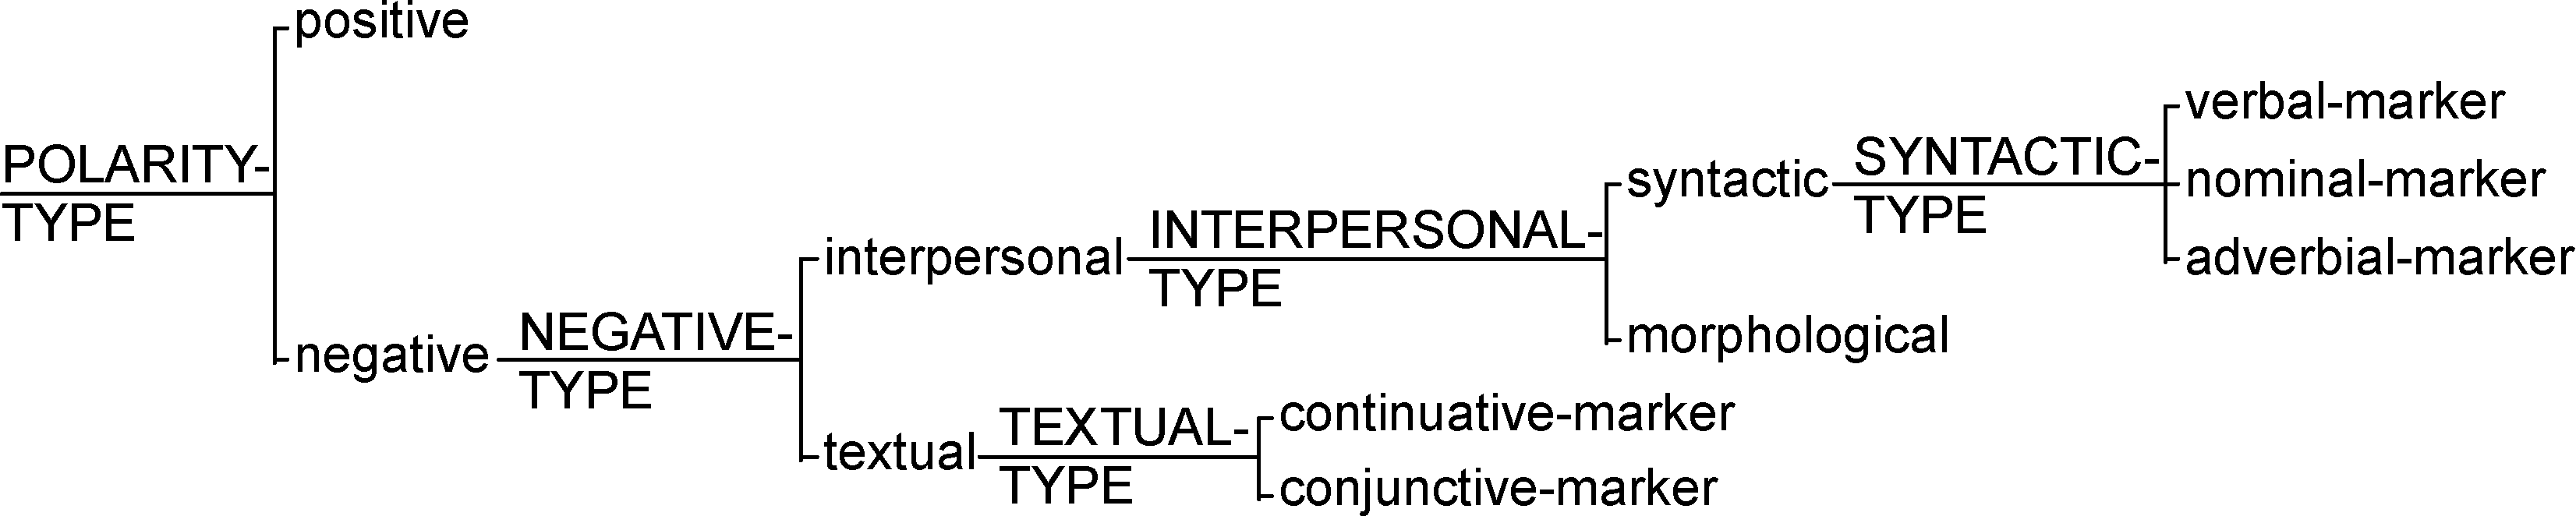
\includegraphics[width=\textwidth]{Figures/SFL-grammar/polarity-system.pdf}
\caption{Polarity System}
\label{fig:polarity1}
\end{figure}

Take for instance the POLARITY system in Figure \ref{fig:polarity1}. Its default selection is \textit{positive} feature unless there is a negative marker. So we must asses NEGATIVE-TYPE system to resolve POLARITY system. But NEGATIVE-TYPE also must be postponed because we do not know if there is a negative marker unless we run tests for each marker type (i.e. presence of a ``no'' particle, negative subject or adjunct etc.). So we postpone selection decision and activate further the INTERPERSONAL-TYPE and TEXTUAL-TYPE systems and base the assessment on the selections yielded by the latter two systems. The same story is with INTERPERSONAL-TYPE which can make selections based on what SYNTACTIC-TYPE system yields. If SYNTACTIC-TYPE and TEXTUAL-TYPE systems yield no selection then we return recursively to INTERPERSONAL-TYPE and to NEGATIVE-TYPE and yield no selection in those systems as well. However if, for instance, \textit{verbal-marker} is detected in the clause then the \textit{syntactic} feature is yielded by the INTERPERSONAL-TYPE and \textit{interpersonal} by the NEGATIVE-TYPE and thus \textit{negative} is yielded by the POLARITY-TYPE. 

Moreover the negative markers can be of various types and more than one can occur simultaneously without any interdependence between them so the algorithm needs to check presence of every type of negative marker i.e. verbal, nominal adverbial, conjunctive and continuative markers. 

That being said the intermediary systems and features i.e. interpersonal, textual, syntactic, morphological are there for the classification purpose only and do not carry any particular algorithmic value making the network from Figure \ref{fig:polarity1} reducible to the one in Figure \ref{fig:polarity1-condensed}. 

\begin{figure}[H]
\centering
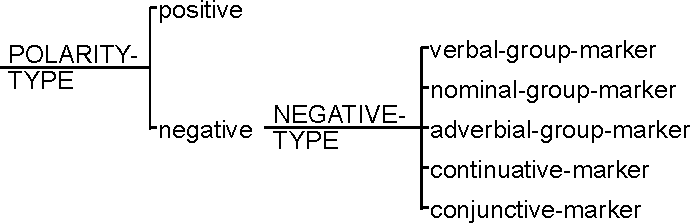
\includegraphics[width=0.6\textwidth]{Figures/SFL-grammar/polarity-condensed.pdf}
\caption{Condensed Polarity System}
\label{fig:polarity1-condensed}
\end{figure}

Execution of system networks is subject to constituent \textit{enrichment phase} of the parsing algorithm. Reducing the POLARITY network to the one in Figure \ref{fig:polarity1-condensed} would lead to loss of information which may be relevant for choice-making in other systems (e.g. MODALITY) so it is useful to expand the selection set with dependent features to achieve feature rich constituents.
